\documentclass[a4paper,11pt,fleqn]{article}%fleqn pour aligner les equations à gauche
\usepackage{/home/rweye/Documents/Overleaf/Styles/Exercice}


\newcommand{\chnum}{Chapitre 6}
\newcommand{\chtitle}{Evolution spontanée d'un système chimique}
\newcommand{\dtype}{Exercices corrigés}

\begin{document}
	\maketitle
\section*{Exercice 1 : Calcul d'un quotient de réaction}
Les ions iodure \ce{I^{-}(aq)}, en contact avec les ions peroxodisulfate \ce{S2O8^{2-}(aq)}, subissant une oxydation lente. On s'intéresse au mélange de \num{100} \unit{\milli \liter} d'une solution de peroxodisulfate d'ammonium (\ce{2 NH4^{+}(aq)} ;\ce{S2O8^{2-}(aq)}) de concentration $c_1$ = \num{0,10} \unit{\mole \per \liter} avec \num{100} \unit{\milli \liter} de solution d'iodure de potassium (\ce{K^{+}(aq)} ; \ce{I^{-}(aq)}) de concentration $c_2$ = \num{0,20} \unit{\mole \per \liter}.
\begin{enumerate}
	\item Établir l'équation de la réaction à partir des couples fournis.\\
	\textcolor{blue}{Équation de la réaction :
	\begin{gather*}
	\ce{ 2 I^{-}(aq) = I2(aq) + 2 e-} \\
	\ce{S2O8^{2-}(aq) + 2 e- = 2 SO4^{2-}(aq) }\\
	\hline
	\ce{S2O8^{2-}(aq) + 2 e- + 2 I^{-}(aq) <=> 2 SO4^{2-}(aq) + I2(aq) + 2 e-} \\
	\ce{S2O8^{2-}(aq) + 2 I^{-}(aq) <=> 2 SO4^{2-}(aq) + I2(aq)}
	\end{gather*}}
	\item Exprimer le quotient de réaction $Q_r$.\\
	\textcolor{blue}{Le quotient de réaction $Q_r$ s'écrit :\\
	$Q_r = \dfrac{\left(\dfrac{[\ce{SO4^{2-}}]}{c^0}\right)^2 \times \left(\dfrac{[\ce{I2}]}{c^0}\right)}{\left(\dfrac{[\ce{S2O8^{2-}}]}{c^0}\right) \times \left(\dfrac{[\ce{I-}]}{c^0}\right)^2} = \dfrac{[\ce{SO4^{2-}}]^2 \times [\ce{I2}]}{[\ce{S2O8^{2-}}] \times [\ce{I-}]^2}$}
	\item Calculer sa valeur à l'état initial.\\
	\textcolor{blue}{À l'état initial on a $Q_{r,i}$ :\\
	$Q_{r,i} = \dfrac{[\ce{SO4^{2-}}]_i^2 \times [\ce{I2}]_i}{[\ce{S2O8^{2-}}]_i \times [\ce{I-}]_i^2} = \dfrac{0 \times 0}{\left(\dfrac{C_1 \times V}{V_{tot}}\right)^2 \times\left(\dfrac{C_2 \times V}{V_{tot}}\right)^2} = 0$  }
\end{enumerate}
La constante d'équilibre de cette réaction est égale à $K$ = \num{2e46}.
\begin{enumerate}
\setcounter{enumi}{3}
	\item Conclure quant au caractère total ou non de la réaction.\\
	\textcolor{blue}{La constante d'équilibre vaut \num{2e46}, cette valeur est bien supérieure à \num{10000} donc la réaction peut être considérée dotale dans le sens direct. On pourra donc écrire l'équation sous la forme : \ce{S2O8^{2-}(aq) + 2 I^{-}(aq) -> 2 SO4^{2-}(aq) + I2(aq)}}
\end{enumerate}
\textbf{Données :}\\
Couples d'oxydoréduction : \ce{I2(aq) / I^{-}(aq)} et \ce{S2O8^{2-}(aq) / SO4^{2-}(aq)}

\section*{Exercice 2 : Calcul de la constante d'équilibre}
L'acide ascorbique \ce{C6H8O6}, plus connu sous le nom de vitamine C, réagit avec l'eau selon l'équation : \\
\ce{C6H8O6(aq) +H_2O(l) <=> C6H7O6-(aq) + H3O+(aq)}\\
À l'équilibre, les concentrations sont les suivantes :
\begin{itemize*}
	\item $[\ce{C6H8O6}]$ = \num{2,6e-1} \unit{\mole \per \liter}
	\item $[\ce{C6H7O6^{-}}]$ = \num{3,1e-3} \unit{\mole \per \liter}
	\item $[\ce{H3O^{+}}]$ = \num{6,7e-3} \unit{\mole \per \liter}
\end{itemize*}
Calculer la constante d'équilibre $K$ de cette réaction.\\
\textcolor{blue}{ $$ Q_{r,eq} = K =  \dfrac{\left(\dfrac{[\ce{C6H7O6-}]}{c^0}\right) \times \left(\dfrac{[\ce{H3O+}]}{c^0}\right)}{\left(\dfrac{[\ce{C6H8O6}]}{c^0}\right)}$$
$$K =  \dfrac{[\ce{C6H7O6-}]_{eq} \times [\ce{H3O+}]_{eq}}{[\ce{C6H8O6}]_{eq}}$$
\fbox{AN :} $K =  \dfrac{\num{3,1e-3} \times\num{6,7e-3}}{\num{2,6e-1}} = \num{8.0e-5}$}

\section*{Exercice 3 : Accident domestique}
L'eau de Javel est une solution aqueuse contenant des ions chlorure \ce{Cl^{-}(aq)}, des ions hypochlorite \ce{ClO^{-}(aq)} et des ions sodium \ce{Na^{+}(aq)}. Mélangé à une solution acide contenant des ions oxonium \ce{H3O^{+}(aq)}, ce produit ménager peut réagir selon l'équation suivante :\\
\ce{ClO^{-}(aq) + Cl^{-}(aq) + 2 H3O^{+}(aq) <=> Cl2(aq) + 2 H2O(l)}
\begin{enumerate}
	\item Exprimer le quotient de réaction $Q_r$\\
	\textcolor{blue}{Le quotient de réaction $Q_r$ s'écrit :\\
	$Q_r = \dfrac{\left(\dfrac{[\ce{Cl2}]}{c^0}\right)}{\left(\dfrac{[\ce{ClO-}]}{c^0}\right) \times \left(\dfrac{[\ce{Cl-}]}{c^0}\right)\times \left(\dfrac{[\ce{H3O+}]}{c^0}\right)^2} =\dfrac{[\ce{Cl2}] }{[\ce{ClO-}] \times [\ce{Cl-}]\times [\ce{H3O+}]^2}$
	}
	\item Compte tenu de la constante d'équilibre fournie, et en supposant que tout le dichlore \ce{Cl2(aq)} formé reste en solution, calculer la quantité de dichlore formé \ce{Cl2(aq)} pour \num{2,0} \unit{\gram} d'ions hypochlorite \ce{ClO-(aq)} réagissant avec les ions oxonium \ce{H3O+(aq)} et chlorure \ce{Cl-(aq)} en excès.\\
	\textcolor{blue}{En se basant sur la valeur de la constante d'équilibre, nous pouvons considérer que la réaction est totale. Ainsi, en se basant sur les données, \ce{ClO-} est le réactif limitant. On pourra ainsi dire que $n_i(\ce{ClO-}) = n_f(\ce{Cl2})$. Soit $$n_f(\ce{Cl2}) = \dfrac{m(\ce{ClO-})}{M(\ce{ClO-})}$$ \fbox{AN :} $n_f(\ce{Cl2}) = \dfrac{\num{2.0}}{\num{35.5}+\num{16.0}}=\SI{3.88E-2}{\mole}$}
	\item Le dichlore \ce{Cl2(aq)} en solution passe rapidement dans l'air, ce qui diminue sa concentration en solution. En déduire le sens d'évolution de la réaction.\\
	\textcolor{blue}{En passant dans l'air, le dichlore formé dans le milieu s'en soustrait. Donc la concentration en \ce{Cl2(aq)} diminue, ce qui va déplacer la valeur du quotient de réaction en le diminuant.}
	\item Expliquer le danger à nettoyer ses toilettes en y versant de l'acide chlorhydrique puis de l'eau de Javel.\\
	\textcolor{blue}{Puisque le dichlore passe sous forme gazeuse, la réaction va continuer de former du dichlore aqueux pour tendre vers l'équilibre. Il y aura donc de plus en plus de dichlore gazeux produit par le mélange réactionnel. Le dichlore étant toxique pour les voies respiratoires, l'utilisation d'eau de Javel en milieu acide est une source de danger.}
\end{enumerate}
\textbf{Données :}\\
\begin{itemize}
	\item Volume molaire à \num{20} \unit{\celsius} sous \num{1,013} \unit{\hecto \pascal} : $V_m$ = \num{24} \unit{\liter \per \mole}
	\item Constante d'équilibre : $K$ = \num{3,2e5}
\end{itemize}

\section*{Exercice 4 : Odeur tropicale}
Le méthanoate d'éthyle \ce{C3H6O2} est un ester présentant une odeur de rhum. Il est utilisé dans l'industrie alimentaire pour parfumer des aliments sans avoir à les alcooliser directement avec du rhum. L'acide méthanoïque \ce{HCOOH} et l'éthanol \ce{C2H6O} sont à l'origine de la synthèse de cet ester.
\begin{enumerate}
	\item Écrire l'équation de la synthèse de cet ester et identifier la seconde espèce chimique produite.\\
	\textcolor{blue}{L'équation de la synthèse de l'ester sera : $$ \ce{ HCOOH + C2H6O = C3H6O2 + H2O}$$ 
	En équilibrant l'équation, on constate qu'il manque deux hydrogène et un oxygène dans les produits ce qui suggère que la seconde espèce chimique produite par cette synthèse est de l'eau.}
\end{enumerate}
Dans un ballon de \num{250} \unit{\milli \liter} sont introduits \num{70} \unit{\milli \liter} d'éthanol de masse volumique $\rho_1$, quatre gouttes de solution d'acide sulfurique concentré \ce{H2SO4(aq)} et quelques grains de pierre ponce. On ajoute \num{45} \unit{\milli \liter} d'acide méthanoïque de masse volumique $\rho_2$. Le mélange est chauffé à reflux jusqu'à obtention de tout l'ester possible. L'état d'équilibre est atteint.
\begin{enumerate}
\setcounter{enumi}{1}
	\item \begin{enumerate}
			\item Préciser le rôle de l'acide sulfurique\\
			\textcolor{blue}{L'acide sulfurique n'entre pas dans l'équation de réaction, il joue le rôle de catalyseur c'est à dire qu'il va augmenter la vitesse de la réaction.}
			\item Identifier le montage à reflux. Nommer l'autre montage.
	\end{enumerate}
\end{enumerate}
\begin{tabular}{>{\centering}m{7cm}>{\centering\arraybackslash}m{9cm}}
Montage 1 & Montage 2\\
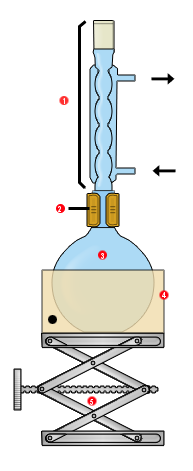
\includegraphics[scale=.5]{Ressources/TSPE_C7_Exercices_Fig1.png}&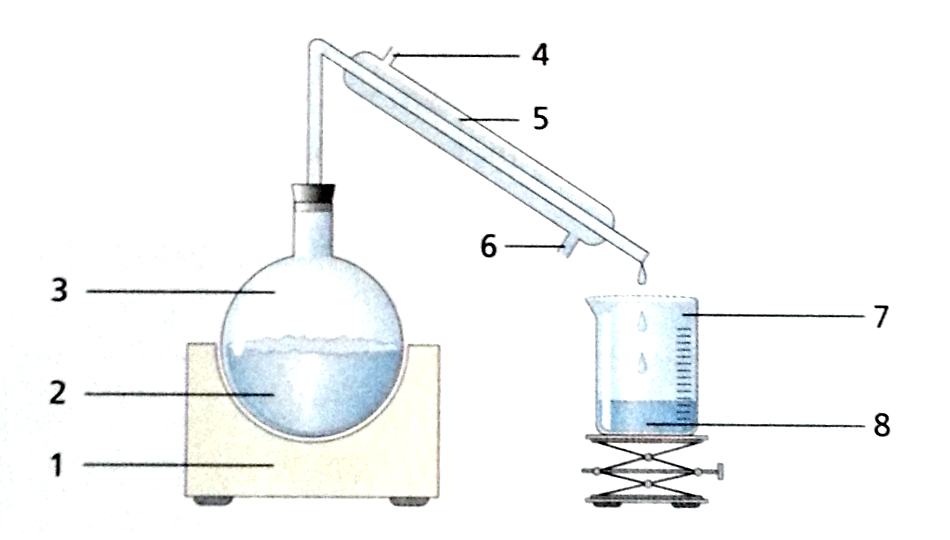
\includegraphics[scale=.3]{Ressources/TSPE_C7_Exercices_Fig2.png}\\
\end{tabular}
\textcolor{blue}{Le montage à reflux est le montage 1, le montage 2 étant une distillation.}
\begin{enumerate}
\setcounter{enumi}{2}
%\setcounter{enumii}{b}
	\item \begin{enumerate}
		\item Réaliser le tableau d'avancement de la réaction\\
		\noindent \textcolor{blue}{
		\begin{tabular}{|>{\centering}m{.15\textwidth}|>{\centering}m{.15\textwidth}|>{\centering}m{.15\textwidth}||>{\centering}m{.15\textwidth}|>{\centering\arraybackslash}m{.15\textwidth}|} \hline
		Avancement &  \ce{HCOOH} & \ce{C2H6O } & \ce{C3H6O2} & \ce{H2O}\\ \hline
		$x=0$ & $n_i(HCOOH) = \dfrac{\rho_2 \cdot V_2}{M(HCOOH)} = \dfrac{\num{1.22} \times \num{45}}{\num{46}} = \SI{1,2}{\mole}$ & $n_i(C2H6O) = \dfrac{\rho_1 \cdot V_1}{M(C2H6O)} = \dfrac{\num{0,789} \times \num{70}}{\num{46}} = \SI{1,2}{\mole}$ & 0 & 0 \\ \hline
		$x=x_f$ & \num{0,4} & \num{0,4} & \num{0,8} & \num{0,8}\\ \hline
		\end{tabular}}
		\item Calculer le taux d'avancement final de la réaction.\\
		\textcolor{blue}{Taux d'avancement : $\tau = \dfrac{x_f}{x_{max}} = \dfrac{0,8}{1,2} = 0,67$\\
		Soit un taux d'avancement de \SI{67}{\percent}.}
	\end{enumerate}
\end{enumerate}
\textbf{Données : }
\begin{itemize*}
	\item Masses volumiques : $\rho_1$ = \num{0,789} \unit{\gram \per \milli \liter} et $\rho_2$ = \num{1,22} \unit{\gram \per \milli \liter} 
	\item Quantités de matière à l'état final : $n(\ce{C3H6O2})$ = \num{0,80} \unit{\mole} et $n(\ce{HCOOH})$ = $n(\ce{C2H6O})$ = \num{0,40} \unit{\mole}
	\item Masses molaires : $M(C)$ = \num{12,0} \unit{\gram \per \mole}, $M(H)$ = \num{1,0} \unit{\gram \per \mole} et $M(O)$ = \num{16,0} \unit{\gram \per \mole}
\end{itemize*}

\section{Tension à vide d'une pile}
Une pile alcaline fonctionne à partir des couples \ce{Zn(s)}/\ce{ZnO(s)} à l'anode et \ce{MnO2(s)}/\ce{Mn2O3(s)} à la cathode.

\begin{enumerate}
    \item Rappeler ce qu'est la tension à vide d'une pile.\\
    \textcolor{blue}{La tension à vide d'une pile est la tension mesurée aux borne de cette pile lorsqu'aucun dipôle n'y est connecté.}
    \item On place un voltmètre aux bornes de la pile, sa borne COM est reliée à la cathode. La tension à vide de cette pile est de \SI{4,5}{\volt}. En déduire la valeur affichée par le voltmètre.\\
    \textcolor{blue}{La cathode d'une pile correspond à son pôle positif, si on y connecte la borne COM du voltmètre, on y lira "$\SI{-4.5}{V}$".}
\end{enumerate}

\section{Vélo électrique}
Une batterie de vélo à assistance électrique a une capacité électrique de \SI{4}{\ampere \hour}. Sur le plat, la batterie débite un courant de \SI{0,5}{\ampere}. En montée, le courant est de \SI{3}{\ampere}.

\begin{enumerate}
    \item Déterminer la durée de fonctionnement de l'assistance électrique sur une route horizontale.\\
    \textcolor{blue}{$$q_{pile} = I \cdot \Delta t$$ $$ \Delta t = \dfrac{q_{pile}}{I} = \dfrac{\num{4}}{\num{0,5}} = \SI{8}{h}$$}
    \item Calculer la durée de fonctionnement de l'assistance pour une route exclusivement en pente ascendante.\\
    \textcolor{blue}{$$q_{pile} = I \cdot \Delta t$$ $$ \Delta t = \dfrac{q_{pile}}{I} = \dfrac{\num{4}}{\num{3}} = \SI{1,3}{h}$$}
\end{enumerate}

\section{Pile cuivre-plomb}
La borne d'entrée d'un voltmètre est reliée à la lame de cuivre \ce{Cu(s)} et la borne COM à la lame de plomb \ce{Pb(s)}.

\begin{figure}[H]
    \centering
    \adjustbox{valign=b}{\subfloat[\textbf{Pile cuivre-plomb}]{
    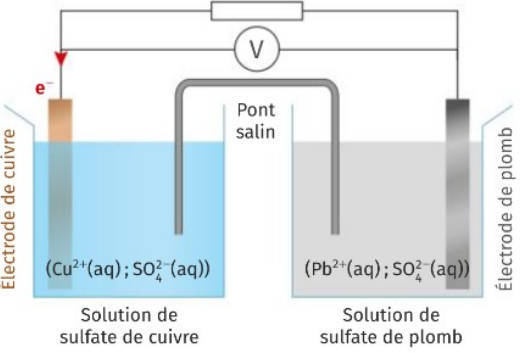
\includegraphics[scale=.5]{Ressources/TSPE_C16_Exercices_Fig1.png}}}
\end{figure}

\begin{enumerate}
    \item Déterminer le sens du courant.\\
    \textcolor{blue}{On observe le sens des électrons vers l'électrode de cuivre, le sens du courant étant contraire à celui des électrons, il ira donc de l'électrode de cuivre vers l'électrode de plomb.}
    \item Identifier l'anode et la cathode.\\
    \textcolor{blue}{L'anode est le siège de l'oxydation, qui libère des électrons ce qui correspond à l'électrode de plomb. La cathode est le siège de la réduction, là où se dirigent les électrons c'est à dire l'électrode de cuivre.}
    \item À l'aide du schéma, écrire les demi-équations d'oxydoréduction.\\
    \textcolor{blue}{Demi équations mises en jeu  : $$ \ce{Pb(s) =Pb^2+(aq) + 2 e-}$$ $$ \ce{Cu^2+(aq) + 2e- = Cu(s)}$$}
    \item En déduire l'équation de fonctionnement de la pile.\\
    \textcolor{blue}{Équation de fonctionnement de la pile : $$ \ce{Pb(s) + Cu^2+(aq) = Cu(s) + Pb^2+(aq)}$$}
\end{enumerate}

\section{Pile nickel-argent}
Une pile nickel argent met en jeu les couples \ce{Ag+(aq)}/\ce{Ag(s)} et \ce{Ni^{2+}(aq)}/\ce{Ni(s)}. Dans la pile, c'est le nickel \ce{Ni(s)} qui s'oxyde.

\begin{enumerate}
    \item Identifier l'anode et la cathode.\\
    \textcolor{blue}{Si l'électrode de nickel s'oxyde, il s'agit de l'anode. L'électrode d'argent jouera donc le rôle de cathode.}
    \item Écrire les demi-équations d'oxydoréduction.\\
    \textcolor{blue}{Demi-équations : $$\ce{Ni(s) = Ni^2+(aq) + 2e-}$$ $$\ce{Ag+(aq) + e- = Ag(s)}$$}
    \item En déduire l'équation globale de la réaction de la pile.\\
    \textcolor{blue}{$$\ce{Ni(s) + 2Ag+(aq) = Ni^2+(aq) + 2Ag(s)}$$}
    \item Donner la relation entre la capacité électrique, l'intensité du courant et la durée de fonctionnement d'une pile.\\
    \textcolor{blue}{$$q_{pile} = I \cdot \Delta t$$}
    \item Rappeler la relation entre la capacité électrique et la quantité de matière d'électrons échangés.\\
    \textcolor{blue}{$$q_{pile} = n_{\ce{e-},ech,max} \cdot F$$}
    \item Calculer la variation de masses de l'anode lorsque la pile a débité un courant continu d'intensité \SI{500}{\milli\ampere} pendant \SI{4,0}{\hour}.\\
    \textcolor{blue}{On peut lier la charge consommée par la pile pendant sa durée de fonctionnement et la quantité de matière d'électrons échangés : $$I \cdot \Delta t = n_{\ce{e-},ech,max} \cdot F$$
    $$n_{\ce{e-},ech,max} = \dfrac{I \cdot \Delta t}{F} = \dfrac{\num{0,5} \cdot \num{4} \times 3600}{\num{9,65E4}}  = \SI{7,5E-2}{\mole}$$
    La quantité d'électrons échangée correspond à deux fois la quantité de matière de nickel oxydée à l'anode. On aura alors : $$n_{Ni, oxyde} = 1/2 \cdot n_{\ce{e-},ech,max} = \SI{3,7E-2}{\mole}$$
    La masse perdue par l'électrode de nickel : $$ m = n_{Ni, oxyde} \cdot M(Ni) = \num{3,7E-2} \times \num{58,7} = \SI{2,2}{\gram}$$}
\end{enumerate}

\begin{figure}[H]
    \begin{minipage}{\linewidth}
     \textbf{Données :}
     \begin{itemize}
        \item \textbf{Masses molaires atomiques :}\\
        $M(\ce{Ag})$ = \SI{107,9}{\gram\per\mole} et $M(\ce{Ni})$ = \SI{58,7}{\gram\per\mole}
        \item \textbf{Constante de Faraday :}\\ $F$ = \SI{9,65E4}{\coulomb\per\mole}
    \end{itemize}
    \end{minipage}
\end{figure}

\section{Vitamine C}
L'acide ascorbique \ce{C6H8O6}, dont l'énantiomère L-ascorbique est connu sous le nom de vitamine C, réagit avec l'eau selon l'équation suivante :
$$\ce{C6H8O6(aq) + H2O(l) <=> C6H7O6-(aq) + H3O+(aq)}$$
La constante d'équilibre de la réaction est égale à $K$ = \num{7,9E-5}.

\begin{enumerate}
    \item Préciser la nature de la réaction.\\
    \textcolor{blue}{Il s'agit d'une réaction acide-base car l'espèce échangée est un \ce{H+}.}
\end{enumerate}
Un comprimé contenant \SI{3,0E-3}{\mole} de vitamine C est dissous sans \SI{200}{\milli\liter} d'eau contenant déjà des ions \ce{C6H7O6-(aq)} à la concentration $[\ce{C6H7O6-}]_i$ = \SI{0,10}{\mole\per\liter}.
\begin{enumerate}[resume]
    \item Avant réaction, déterminer la concentration initiale d'acide ascorbique \ce{C6H8O6(aq)}.\\
    \textcolor{blue}{$[\ce{C6H8O6}]_i = \dfrac{n(\ce{C6H8O6})}{V} = \dfrac{\num{3,0E-3}}{0,2} = \SI{1,5E-2}{\mole\per\liter}$}
    \item En déduire le sens d'évolution spontanée de cette réaction.\\
    \textcolor{blue}{Pour déduire le sens d'évolution de la réaction, on compare la valeur de $Q_{r,i}$ à $K$.
    $$Q_{r,i} = \dfrac{[\ce{C6H7O6-}]_i \cdot [\ce{H3O+}]_i}{[\ce{C6H8O6}]_i}$$
    $$Q_{r,i} = \dfrac{\num{0,1} \times 10^{-7,8}}{\num{1,5E-2}}= \num{1,06E-7}$$}
\end{enumerate}
\begin{figure}[H]
    \begin{minipage}{\linewidth}
    \textbf{Donnée :}
    \begin{itemize}
        \item \textbf{pH de la solution avant dissolution du comprimé :} pH = \num{7,8}
    \end{itemize}
    \end{minipage}
\end{figure}

\section{Question de taille}
L'équation de la réaction d'une pile cuivre-zinc est :
$$\ce{Zn(s) + Cu^{2+}(aq) <=> Cu(s) + Zn^{2+}(aq)}$$
La lame de zinc constitue l'anode.
\begin{enumerate}
    \item Écrire les demi-équations associées.\\
    \textcolor{blue}{Demi-équations : $$\ce{Zn(s) = Zn^2+(aq) + 2e-}$$ $$\ce{Cu^2+(aq) +2e- = Cu(s)}$$}
    \item Exprimer la quantité de matière d'électrons transférés.\\
    \textcolor{blue}{$$n_{\ce{e-},ech} = 2 \cdot n_{Zn\text{, consommé}} = 2 \cdot n_{Cu\text{, formé}}$$}
    \item Calculer la capacité électrique de cette pile.\\
    \textcolor{blue}{$$q_{pile} = n_{\ce{e-},ech, max} \cdot F$$
    Pour estimer la quantité de matière maximale d'électron échangés, il faut estimer le réactif limitant, sans informations sur les solutions, on considèrera que le réactif limitant est la lame de zinc.\\ $n_i(Zn) = \dfrac{m_{anode}}{M(Zn)} = \dfrac{\num{8,0}}{\num{65,4}} = \SI{0,12}{mol}$\\
    On aura donc :
    $$q_{pile} = n_{\ce{e-},ech, max} \cdot F = 2 \cdot n_{i}(Zn) \cdot F$$
    $$q_{pile} = 2 \times \num{0,12} \times \num{9,65E4} = \SI{2,3E4}{C}$$}
    \item Les masse de chaque électrode sont doublées. Calculer la nouvelle capacité électrique.\\
    \textcolor{blue}{En doublant toutes les quantités on aura :
    $$q_{pile} = n_{\ce{e-},ech, max} \cdot F = 4 \cdot n_{i}(Zn) \cdot F$$
    $$q_{pile} = 4 \times \num{0,12} \times \num{9,65E4} = \SI{4,6E4}{C}$$
    La capacité de la pile aura doublé.}
    \item Conclure quant à l'influence de la masse de l'anode et de la cathode.\\
    \textcolor{blue}{Dans le cadre d'une pile, la masse de l'anode aura une importance directe sur la capacité de celle-ci, elle doit être maximale pour augmenter la capacité. La masse de la cathode n'entre pas en compte dans la détermination de la capacité.}
\end{enumerate}
\begin{figure}[H]
    \begin{minipage}{\linewidth}
    \textbf{Donnée :}
    \begin{itemize}
        \item \textbf{Masses des électrodes :} $m_{anode}$ = \SI{8,0}{\gram} et $m_{cathode}$ = \SI{6,0}{\gram}
        \item \textbf{Constante de Faraday :} $F$ = \SI{9,65E4}{\coulomb\per\mole}
        \item \textbf{Masses molaires :} $M(\ce{Zn})$ = \SI{65,4}{\gram\per\mole} et $M(\ce{Cu})$ = \SI{63,5}{\gram\per\mole}
    \end{itemize}
    \end{minipage}
\end{figure}

\section{Pile citron}
Un moyen simple de réaliser une pile est de planter un trombone recouvert de zinc et une pièce recouverte de cuivre dans un citron.\\
Une lampe, reliée d'un coté au trombone et de l'autre à la pile, s'allume. Un voltmètre branché à la pile citron affiche \SI{0,84}{\volt}. Sa borne V est du coté du cuivre, la borne COM est reliée au trombone.
\begin{enumerate}
    \item Préciser ce que représente la valeur mesurée.\\
    \textcolor{blue}{La valeur mesurée représente la tension à vide de la pile.}
    \item Déterminer la polarité de la pile au niveau du trombone et de la pièce. Justifier.\\
    \textcolor{blue}{La tension à vide est positive indiquant que la borne V est reliée à la cathode (positive) et la borne COM à l'anode (négative).}
\end{enumerate}
Au cours de l'utilisation de la pile, du dihydrogène \ce{H2(g)} se dégage.
\begin{enumerate}[resume]
    \item Écrire les demi-équations d'oxydoréduction ayant lieu à chaque électrode.\\
    \textcolor{blue}{Demi-équations : $$\text{Cathode : }\ce{2H+(aq) + 2e- = H2(g)}$$
    $$\text{Anode : }\ce{Zn(s) = Zn^2+(aq) + 2e-}$$}
    \item En déduire l'équation de réaction globale de la pile citron.\\
    \textcolor{blue}{Équation globale : $$\ce{Zn(s) + 2H+(aq) = Zn^2+(aq) + H2(g)}$$}
    \item Préciser d'où proviennent les ions \ce{H+(aq)}.\\
    \textcolor{blue}{Les ions \ce{H+(aq)} proviennent naturellement du jus de citron qui est connu pour son acidité, donc sa concentration importante en ions \ce{H+(aq)}.}
    \item Toujours à partir de citrons, trombones et pièces de cuivre, proposer un dispositif délivrant une tension deux fois plus grande.\\
    \textcolor{blue}{Pour augmenter la tension, sans changer les couples mis en jeux on peut augmenter les quantités de matières dans les espèces, en particulier en travaillant avec une acidité plus importante.}
\end{enumerate}

\begin{figure}[H]
    \begin{minipage}{\linewidth}
    \textbf{Donnée :}
    \begin{itemize}
        \item \textbf{Couples d'oxydoréduction :} \ce{Zn^{2+}(aq)}/\ce{Zn(s)} et \ce{H+(aq)}/\ce{H2(g)}
    \end{itemize}
    \end{minipage}
\end{figure}

\section{Pile cuivre-aluminium}
Une pile est composée de deux demi-piles reliées par un papier filtre imbibé d'une solution de chlorure de potassium (\ce{K+(aq)} ; \ce{Cl-(aq)}). La première demi-pile est constituée d'une lame d'aluminium de masse $m_1$ = \SI{1,0}{\gram} qui plonge dans \SI{50}{\milli\liter} de solution de sulfate d'aluminium (\ce{2Al^{3+}(aq)} ; \ce{3SO4^{2-}(aq)}) de concentration en ion aluminium \ce{Al^{3+}(aq)} égale à $[\ce{Al^{3+}}]$ = \SI{5,0E-1}{\mole\per\liter}.\\
La seconde est constituée d'une lame de cuivre de masse $m_2$ = \SI{8,9}{\gram} qui plonge dans \SI{50}{mL} de solution de sulfate de cuivre (\ce{Cu^{2+}(aq)};\ce{SO4^{2-}(aq)}) de concentration en ion cuivre \ce{Cu^{2+}(aq)} égale à $[\ce{Cu^{2+}}]$ = \SI{5,0E-1}{\mole\per\liter}. Un ampèremètre indique qu'à l'extérieur de la pile, le courant circule de la plaque de cuivre vers la plaque d'aluminium.
\begin{enumerate}
    \item Rappeler le rôle du papier filtre.
    \item Préciser le sens de déplacement des électrons.
    \item Indiquer quelle lame est l'anode.
    \item Réaliser le schéma annoté de la pile.
\end{enumerate}
L'équation de fonctionnement de la pile est :
$$\ce{3 Cu^{2+}(aq) + 2 Al(s) <=> 3 Cu(s) + 2 Al^{3+}(aq)}$$
\begin{enumerate}[resume]
    \item Écrire les demi-équations  d'oxydoréduction de chaque électrode.
\end{enumerate}
La constante d'équilibre associée à l'équation précédente est $K$ = $10^{200}$.
\begin{enumerate}[resume]
    \item \begin{enumerate}
        \item Exprimer puis calculer la valeur du quotient de la réaction $Q_{r,i}$ à l'état initial.
        \item Conclure  quant à la cohérence du sens d'évolution attendu.
    \end{enumerate}
    \item Faire le bilan des quantités de matière du système chimique à l'état initial.
    \item Établir le tableau d'avancement de la réaction de manière littérale.
    \item En déduire la valeur de l'avancement maximal $x_{max}$.
    \item Calculer la capacité électrique que peut débiter cette pile.
\end{enumerate}
\begin{figure}[H]
    \begin{minipage}{\linewidth}
    \textbf{Donnée :}
    \begin{itemize}
        \item \textbf{Masses molaires atomiques :} $M(\ce{Al})$ = \SI{27,0}{\gram\per\mole} et $M(\ce{Cu})$ = \SI{63,5}{\gram\per\mole}
        \item \textbf{ Couples d'oxydoréduction :} \ce{Cu^{2+}(aq)}/\ce{Cu(s)} et \ce{Al^{3+}(aq)}/\ce{Al(s)}
    \end{itemize}
    \end{minipage}
\end{figure}

\end{document}